\documentclass{book}
\usepackage[a4paper,top=2.5cm,bottom=2.5cm,left=2.5cm,right=2.5cm]{geometry}
\usepackage{makeidx}
\usepackage{natbib}
\usepackage{graphicx}
\usepackage{multicol}
\usepackage{float}
\usepackage{listings}
\usepackage{color}
\usepackage{ifthen}
\usepackage[table]{xcolor}
\usepackage{textcomp}
\usepackage{alltt}
\usepackage{ifpdf}
\ifpdf
\usepackage[pdftex,
            pagebackref=true,
            colorlinks=true,
            linkcolor=blue,
            unicode
           ]{hyperref}
\else
\usepackage[ps2pdf,
            pagebackref=true,
            colorlinks=true,
            linkcolor=blue,
            unicode
           ]{hyperref}
\usepackage{pspicture}
\fi
\usepackage[utf8]{inputenc}
\usepackage{mathptmx}
\usepackage[scaled=.90]{helvet}
\usepackage{courier}
\usepackage{sectsty}
\usepackage{amssymb}
\usepackage[titles]{tocloft}
\usepackage{doxygen}
\lstset{language=C++,inputencoding=utf8,basicstyle=\footnotesize,breaklines=true,breakatwhitespace=true,tabsize=4,numbers=left }
\makeindex
\setcounter{tocdepth}{3}
\renewcommand{\footrulewidth}{0.4pt}
\renewcommand{\familydefault}{\sfdefault}
\hfuzz=15pt
\setlength{\emergencystretch}{15pt}
\hbadness=750
\tolerance=750
\begin{document}
\hypersetup{pageanchor=false,citecolor=blue}
\begin{titlepage}
\vspace*{7cm}
\begin{center}
{\Large Challenger 604 Systems Logic }\\
\vspace*{1cm}
{\large Generated by Doxygen 1.8.2}\\
\vspace*{0.5cm}
{\small Fri Oct 19 2012 21:33:55}\\
\end{center}
\end{titlepage}
\clearemptydoublepage
\pagenumbering{roman}
\tableofcontents
\clearemptydoublepage
\pagenumbering{arabic}
\hypersetup{pageanchor=true,citecolor=blue}
\chapter{Namespace Index}
\section{Namespace List}
Here is a list of all documented namespaces with brief descriptions\-:\begin{DoxyCompactList}
\item\contentsline{section}{\hyperlink{namespace_challenger604_systems}{Challenger604\-Systems} \\*This namespace contains everything in this project }{\pageref{namespace_challenger604_systems}}{}
\end{DoxyCompactList}

\chapter{Hierarchical Index}
\section{Class Hierarchy}
This inheritance list is sorted roughly, but not completely, alphabetically\-:\begin{DoxyCompactList}
\item Q\-Object\begin{DoxyCompactList}
\item \contentsline{section}{Challenger604\-Systems\-:\-:Power\-Source}{\pageref{class_challenger604_systems_1_1_power_source}}{}
\begin{DoxyCompactList}
\item \contentsline{section}{Challenger604\-Systems\-:\-:A\-C\-Power\-Source}{\pageref{class_challenger604_systems_1_1_a_c_power_source}}{}
\begin{DoxyCompactList}
\item \contentsline{section}{Challenger604\-Systems\-:\-:Simple\-A\-C\-Power\-Source}{\pageref{class_challenger604_systems_1_1_simple_a_c_power_source}}{}
\end{DoxyCompactList}
\item \contentsline{section}{Challenger604\-Systems\-:\-:Simple\-D\-C\-Power\-Source}{\pageref{class_challenger604_systems_1_1_simple_d_c_power_source}}{}
\begin{DoxyCompactList}
\item \contentsline{section}{Challenger604\-Systems\-:\-:A\-P\-U}{\pageref{class_challenger604_systems_1_1_a_p_u}}{}
\end{DoxyCompactList}
\end{DoxyCompactList}
\end{DoxyCompactList}
\end{DoxyCompactList}

\chapter{Class Index}
\section{Class List}
Here are the classes, structs, unions and interfaces with brief descriptions\-:\begin{DoxyCompactList}
\item\contentsline{section}{\hyperlink{class_challenger604_systems_1_1_a_c_power_source}{Challenger604\-Systems\-::\-A\-C\-Power\-Source} }{\pageref{class_challenger604_systems_1_1_a_c_power_source}}{}
\item\contentsline{section}{\hyperlink{class_challenger604_systems_1_1_a_p_u}{Challenger604\-Systems\-::\-A\-P\-U} }{\pageref{class_challenger604_systems_1_1_a_p_u}}{}
\item\contentsline{section}{\hyperlink{class_challenger604_systems_1_1_aural_warning_system}{Challenger604\-Systems\-::\-Aural\-Warning\-System} \\*A class for an aural warning system }{\pageref{class_challenger604_systems_1_1_aural_warning_system}}{}
\item\contentsline{section}{\hyperlink{class_challenger604_systems_1_1_c_a_s_1_1_c_a_s_advisory_message}{Challenger604\-Systems\-::\-C\-A\-S\-::\-C\-A\-S\-Advisory\-Message} \\*A \hyperlink{namespace_challenger604_systems_1_1_c_a_s}{C\-A\-S} message with a priority level of A\-D\-V\-I\-S\-O\-R\-Y }{\pageref{class_challenger604_systems_1_1_c_a_s_1_1_c_a_s_advisory_message}}{}
\item\contentsline{section}{\hyperlink{class_challenger604_systems_1_1_c_a_s_1_1_c_a_s_caution_message}{Challenger604\-Systems\-::\-C\-A\-S\-::\-C\-A\-S\-Caution\-Message} \\*A \hyperlink{namespace_challenger604_systems_1_1_c_a_s}{C\-A\-S} message with a priority level of C\-A\-U\-T\-I\-O\-N }{\pageref{class_challenger604_systems_1_1_c_a_s_1_1_c_a_s_caution_message}}{}
\item\contentsline{section}{\hyperlink{class_challenger604_systems_1_1_c_a_s_1_1_c_a_s_message}{Challenger604\-Systems\-::\-C\-A\-S\-::\-C\-A\-S\-Message} \\*Base class for a Crew Alerting System message }{\pageref{class_challenger604_systems_1_1_c_a_s_1_1_c_a_s_message}}{}
\item\contentsline{section}{\hyperlink{class_challenger604_systems_1_1_c_a_s_1_1_c_a_s_status_message}{Challenger604\-Systems\-::\-C\-A\-S\-::\-C\-A\-S\-Status\-Message} \\*A \hyperlink{namespace_challenger604_systems_1_1_c_a_s}{C\-A\-S} message with a priority level of S\-T\-A\-T\-U\-S }{\pageref{class_challenger604_systems_1_1_c_a_s_1_1_c_a_s_status_message}}{}
\item\contentsline{section}{\hyperlink{class_challenger604_systems_1_1_c_a_s_1_1_c_a_s_warning_message}{Challenger604\-Systems\-::\-C\-A\-S\-::\-C\-A\-S\-Warning\-Message} \\*A \hyperlink{namespace_challenger604_systems_1_1_c_a_s}{C\-A\-S} message with a priority level of W\-A\-R\-N\-I\-N\-G }{\pageref{class_challenger604_systems_1_1_c_a_s_1_1_c_a_s_warning_message}}{}
\item\contentsline{section}{\hyperlink{class_challenger604_systems_1_1_endless_a_c_power_source}{Challenger604\-Systems\-::\-Endless\-A\-C\-Power\-Source} }{\pageref{class_challenger604_systems_1_1_endless_a_c_power_source}}{}
\item\contentsline{section}{\hyperlink{class_challenger604_systems_1_1_fuel_1_1_fuel_sink}{Challenger604\-Systems\-::\-Fuel\-::\-Fuel\-Sink} \\*An interface for anything that consumes fuel. All fuel flow rates, unless otherwise noted, are in kilograms per hour }{\pageref{class_challenger604_systems_1_1_fuel_1_1_fuel_sink}}{}
\item\contentsline{section}{\hyperlink{class_challenger604_systems_1_1_power_sink}{Challenger604\-Systems\-::\-Power\-Sink} \\*Abstract base class for anything that accepts electricity from something else }{\pageref{class_challenger604_systems_1_1_power_sink}}{}
\item\contentsline{section}{\hyperlink{class_challenger604_systems_1_1_power_source}{Challenger604\-Systems\-::\-Power\-Source} }{\pageref{class_challenger604_systems_1_1_power_source}}{}
\item\contentsline{section}{\hyperlink{class_challenger604_systems_1_1_simple_a_c_power_sink}{Challenger604\-Systems\-::\-Simple\-A\-C\-Power\-Sink} }{\pageref{class_challenger604_systems_1_1_simple_a_c_power_sink}}{}
\item\contentsline{section}{\hyperlink{class_challenger604_systems_1_1_simple_a_c_power_source}{Challenger604\-Systems\-::\-Simple\-A\-C\-Power\-Source} }{\pageref{class_challenger604_systems_1_1_simple_a_c_power_source}}{}
\item\contentsline{section}{\hyperlink{class_challenger604_systems_1_1_simple_d_c_power_sink}{Challenger604\-Systems\-::\-Simple\-D\-C\-Power\-Sink} \\*A power sink that accepts D\-C power }{\pageref{class_challenger604_systems_1_1_simple_d_c_power_sink}}{}
\item\contentsline{section}{\hyperlink{class_challenger604_systems_1_1_simple_d_c_power_source}{Challenger604\-Systems\-::\-Simple\-D\-C\-Power\-Source} }{\pageref{class_challenger604_systems_1_1_simple_d_c_power_source}}{}
\item\contentsline{section}{\hyperlink{class_challenger604_systems_1_1_c_a_s_1_1_takeoff_autopilot_engaged_message}{Challenger604\-Systems\-::\-C\-A\-S\-::\-Takeoff\-Autopilot\-Engaged\-Message} \\*A message that is sent when the aircraft is in takeoff configuration but the autopilot is engaged }{\pageref{class_challenger604_systems_1_1_c_a_s_1_1_takeoff_autopilot_engaged_message}}{}
\item\contentsline{section}{\hyperlink{class_challenger604_systems_1_1_c_a_s_1_1_takeoff_flaps_message}{Challenger604\-Systems\-::\-C\-A\-S\-::\-Takeoff\-Flaps\-Message} \\*A warning message that is sent when the aircraft is in takeoff configuration but the flaps are not set }{\pageref{class_challenger604_systems_1_1_c_a_s_1_1_takeoff_flaps_message}}{}
\item\contentsline{section}{\hyperlink{class_challenger604_systems_1_1_test_d_c_power_sink}{Challenger604\-Systems\-::\-Test\-D\-C\-Power\-Sink} \\*A power sink that consumes 100 watts of power at 28 volts D\-C }{\pageref{class_challenger604_systems_1_1_test_d_c_power_sink}}{}
\item\contentsline{section}{\hyperlink{class_challenger604_systems_1_1_t_r_u}{Challenger604\-Systems\-::\-T\-R\-U} }{\pageref{class_challenger604_systems_1_1_t_r_u}}{}
\end{DoxyCompactList}

\chapter{File Index}
\section{File List}
Here is a list of all documented files with brief descriptions\-:\begin{DoxyCompactList}
\item\contentsline{section}{/\-Applications/\-X-\/\-Plane 10 Demo/\-Aircraft/\-Heavy Metal/\-Challenger 604/\-Challenger604\-Logic/{\bfseries Challenger604\-Logic\-\_\-global.\-h} }{\pageref{_challenger604_logic__global_8h}}{}
\item\contentsline{section}{/\-Applications/\-X-\/\-Plane 10 Demo/\-Aircraft/\-Heavy Metal/\-Challenger 604/\-Challenger604\-Logic/electrical/components/{\bfseries apu.\-h} }{\pageref{apu_8h}}{}
\item\contentsline{section}{/\-Applications/\-X-\/\-Plane 10 Demo/\-Aircraft/\-Heavy Metal/\-Challenger 604/\-Challenger604\-Logic/electrical/components/{\bfseries endlessacpowersource.\-h} }{\pageref{endlessacpowersource_8h}}{}
\item\contentsline{section}{/\-Applications/\-X-\/\-Plane 10 Demo/\-Aircraft/\-Heavy Metal/\-Challenger 604/\-Challenger604\-Logic/electrical/components/{\bfseries testdcpowersink.\-h} }{\pageref{testdcpowersink_8h}}{}
\item\contentsline{section}{/\-Applications/\-X-\/\-Plane 10 Demo/\-Aircraft/\-Heavy Metal/\-Challenger 604/\-Challenger604\-Logic/electrical/components/{\bfseries tru.\-h} }{\pageref{tru_8h}}{}
\item\contentsline{section}{/\-Applications/\-X-\/\-Plane 10 Demo/\-Aircraft/\-Heavy Metal/\-Challenger 604/\-Challenger604\-Logic/electrical/defs/{\bfseries acpowersource.\-h} }{\pageref{acpowersource_8h}}{}
\item\contentsline{section}{/\-Applications/\-X-\/\-Plane 10 Demo/\-Aircraft/\-Heavy Metal/\-Challenger 604/\-Challenger604\-Logic/electrical/defs/\hyperlink{electricalpowertype_8h}{electricalpowertype.\-h} \\*Contains an enum for types of electrical power }{\pageref{electricalpowertype_8h}}{}
\item\contentsline{section}{/\-Applications/\-X-\/\-Plane 10 Demo/\-Aircraft/\-Heavy Metal/\-Challenger 604/\-Challenger604\-Logic/electrical/defs/{\bfseries powersink.\-h} }{\pageref{powersink_8h}}{}
\item\contentsline{section}{/\-Applications/\-X-\/\-Plane 10 Demo/\-Aircraft/\-Heavy Metal/\-Challenger 604/\-Challenger604\-Logic/electrical/defs/{\bfseries powersource.\-h} }{\pageref{powersource_8h}}{}
\item\contentsline{section}{/\-Applications/\-X-\/\-Plane 10 Demo/\-Aircraft/\-Heavy Metal/\-Challenger 604/\-Challenger604\-Logic/electrical/defs/{\bfseries simpleacpowersink.\-h} }{\pageref{simpleacpowersink_8h}}{}
\item\contentsline{section}{/\-Applications/\-X-\/\-Plane 10 Demo/\-Aircraft/\-Heavy Metal/\-Challenger 604/\-Challenger604\-Logic/electrical/defs/{\bfseries simpleacpowersource.\-h} }{\pageref{simpleacpowersource_8h}}{}
\item\contentsline{section}{/\-Applications/\-X-\/\-Plane 10 Demo/\-Aircraft/\-Heavy Metal/\-Challenger 604/\-Challenger604\-Logic/electrical/defs/{\bfseries simpledcpowersink.\-h} }{\pageref{simpledcpowersink_8h}}{}
\item\contentsline{section}{/\-Applications/\-X-\/\-Plane 10 Demo/\-Aircraft/\-Heavy Metal/\-Challenger 604/\-Challenger604\-Logic/electrical/defs/{\bfseries simpledcpowersource.\-h} }{\pageref{simpledcpowersource_8h}}{}
\end{DoxyCompactList}

\chapter{Namespace Documentation}
\hypertarget{namespace_challenger604_systems}{\section{Challenger604\-Systems Namespace Reference}
\label{namespace_challenger604_systems}\index{Challenger604\-Systems@{Challenger604\-Systems}}
}


This namespace contains everything in this project.  


\subsection*{Classes}
\begin{DoxyCompactItemize}
\item 
class \hyperlink{class_challenger604_systems_1_1_a_p_u}{A\-P\-U}
\item 
class \hyperlink{class_challenger604_systems_1_1_endless_a_c_power_source}{Endless\-A\-C\-Power\-Source}
\item 
class \hyperlink{class_challenger604_systems_1_1_test_d_c_power_sink}{Test\-D\-C\-Power\-Sink}
\begin{DoxyCompactList}\small\item\em A power sink that consumes 100 watts of power at 28 volts D\-C. \end{DoxyCompactList}\item 
class \hyperlink{class_challenger604_systems_1_1_t_r_u}{T\-R\-U}
\item 
class \hyperlink{class_challenger604_systems_1_1_a_c_power_source}{A\-C\-Power\-Source}
\item 
class \hyperlink{class_challenger604_systems_1_1_power_sink}{Power\-Sink}
\begin{DoxyCompactList}\small\item\em Abstract base class for anything that accepts electricity from something else. \end{DoxyCompactList}\item 
class \hyperlink{class_challenger604_systems_1_1_power_source}{Power\-Source}
\item 
class \hyperlink{class_challenger604_systems_1_1_simple_a_c_power_sink}{Simple\-A\-C\-Power\-Sink}
\item 
class \hyperlink{class_challenger604_systems_1_1_simple_a_c_power_source}{Simple\-A\-C\-Power\-Source}
\item 
class \hyperlink{class_challenger604_systems_1_1_simple_d_c_power_sink}{Simple\-D\-C\-Power\-Sink}
\begin{DoxyCompactList}\small\item\em A power sink that accepts D\-C power. \end{DoxyCompactList}\item 
class \hyperlink{class_challenger604_systems_1_1_simple_d_c_power_source}{Simple\-D\-C\-Power\-Source}
\end{DoxyCompactItemize}
\subsection*{Enumerations}
\begin{DoxyCompactItemize}
\item 
enum \hyperlink{namespace_challenger604_systems_a9ad1a793d94b97514092692cb7315afd}{Electrical\-Power\-Type} \{ \\*
\hyperlink{namespace_challenger604_systems_a9ad1a793d94b97514092692cb7315afdac443cb4f2e9c8fb362d1b23d390680c1}{D\-C\-\_\-\-O\-T\-H\-E\-R}, 
\hyperlink{namespace_challenger604_systems_a9ad1a793d94b97514092692cb7315afdaeb46efa4ea7afd565b7f41c0881a206d}{D\-C\-\_\-12\-V}, 
\hyperlink{namespace_challenger604_systems_a9ad1a793d94b97514092692cb7315afdaa549263d4db7adacf1008dac6a68b21d}{D\-C\-\_\-28\-V}, 
\hyperlink{namespace_challenger604_systems_a9ad1a793d94b97514092692cb7315afda2fcb938b597382142bdc684898fe8596}{A\-C\-\_\-\-O\-T\-H\-E\-R}, 
\\*
\hyperlink{namespace_challenger604_systems_a9ad1a793d94b97514092692cb7315afdade695fe37c4e590d464845feb03fcfde}{A\-C\-\_\-115\-V\-\_\-400\-H\-Z}
 \}
\begin{DoxyCompactList}\small\item\em An enumeration of different types of electricity. Note that all voltage and frequency values here are nominal. The actual values may be different. \end{DoxyCompactList}\end{DoxyCompactItemize}


\subsection{Detailed Description}
This namespace contains everything in this project. 

\subsection{Enumeration Type Documentation}
\hypertarget{namespace_challenger604_systems_a9ad1a793d94b97514092692cb7315afd}{\index{Challenger604\-Systems@{Challenger604\-Systems}!Electrical\-Power\-Type@{Electrical\-Power\-Type}}
\index{Electrical\-Power\-Type@{Electrical\-Power\-Type}!Challenger604Systems@{Challenger604\-Systems}}
\subsubsection[{Electrical\-Power\-Type}]{\setlength{\rightskip}{0pt plus 5cm}enum {\bf Challenger604\-Systems\-::\-Electrical\-Power\-Type}}}\label{namespace_challenger604_systems_a9ad1a793d94b97514092692cb7315afd}


An enumeration of different types of electricity. Note that all voltage and frequency values here are nominal. The actual values may be different. 

\begin{Desc}
\item[Enumerator\-: ]\par
\begin{description}
\index{D\-C\-\_\-\-O\-T\-H\-E\-R@{D\-C\-\_\-\-O\-T\-H\-E\-R}!Challenger604\-Systems@{Challenger604\-Systems}}\index{Challenger604\-Systems@{Challenger604\-Systems}!D\-C\-\_\-\-O\-T\-H\-E\-R@{D\-C\-\_\-\-O\-T\-H\-E\-R}}\item[{\em 
\hypertarget{namespace_challenger604_systems_a9ad1a793d94b97514092692cb7315afdac443cb4f2e9c8fb362d1b23d390680c1}{D\-C\-\_\-\-O\-T\-H\-E\-R}\label{namespace_challenger604_systems_a9ad1a793d94b97514092692cb7315afdac443cb4f2e9c8fb362d1b23d390680c1}
}]D\-C electricity with an unknown voltage \index{D\-C\-\_\-12\-V@{D\-C\-\_\-12\-V}!Challenger604\-Systems@{Challenger604\-Systems}}\index{Challenger604\-Systems@{Challenger604\-Systems}!D\-C\-\_\-12\-V@{D\-C\-\_\-12\-V}}\item[{\em 
\hypertarget{namespace_challenger604_systems_a9ad1a793d94b97514092692cb7315afdaeb46efa4ea7afd565b7f41c0881a206d}{D\-C\-\_\-12\-V}\label{namespace_challenger604_systems_a9ad1a793d94b97514092692cb7315afdaeb46efa4ea7afd565b7f41c0881a206d}
}]D\-C electricity at 12 volts \index{D\-C\-\_\-28\-V@{D\-C\-\_\-28\-V}!Challenger604\-Systems@{Challenger604\-Systems}}\index{Challenger604\-Systems@{Challenger604\-Systems}!D\-C\-\_\-28\-V@{D\-C\-\_\-28\-V}}\item[{\em 
\hypertarget{namespace_challenger604_systems_a9ad1a793d94b97514092692cb7315afdaa549263d4db7adacf1008dac6a68b21d}{D\-C\-\_\-28\-V}\label{namespace_challenger604_systems_a9ad1a793d94b97514092692cb7315afdaa549263d4db7adacf1008dac6a68b21d}
}]D\-C electricty at 28 volts \index{A\-C\-\_\-\-O\-T\-H\-E\-R@{A\-C\-\_\-\-O\-T\-H\-E\-R}!Challenger604\-Systems@{Challenger604\-Systems}}\index{Challenger604\-Systems@{Challenger604\-Systems}!A\-C\-\_\-\-O\-T\-H\-E\-R@{A\-C\-\_\-\-O\-T\-H\-E\-R}}\item[{\em 
\hypertarget{namespace_challenger604_systems_a9ad1a793d94b97514092692cb7315afda2fcb938b597382142bdc684898fe8596}{A\-C\-\_\-\-O\-T\-H\-E\-R}\label{namespace_challenger604_systems_a9ad1a793d94b97514092692cb7315afda2fcb938b597382142bdc684898fe8596}
}]A\-C electricity with an unkown voltage and frequency \index{A\-C\-\_\-115\-V\-\_\-400\-H\-Z@{A\-C\-\_\-115\-V\-\_\-400\-H\-Z}!Challenger604\-Systems@{Challenger604\-Systems}}\index{Challenger604\-Systems@{Challenger604\-Systems}!A\-C\-\_\-115\-V\-\_\-400\-H\-Z@{A\-C\-\_\-115\-V\-\_\-400\-H\-Z}}\item[{\em 
\hypertarget{namespace_challenger604_systems_a9ad1a793d94b97514092692cb7315afdade695fe37c4e590d464845feb03fcfde}{A\-C\-\_\-115\-V\-\_\-400\-H\-Z}\label{namespace_challenger604_systems_a9ad1a793d94b97514092692cb7315afdade695fe37c4e590d464845feb03fcfde}
}]A\-C electricity at 400 hertz with a voltage of 115 volts. This is the primary type of A\-C electricity on the aircraft. \end{description}
\end{Desc}


\chapter{Class Documentation}
\hypertarget{class_challenger604_systems_1_1_a_c_power_source}{\section{Challenger604\-Systems\-:\-:A\-C\-Power\-Source Class Reference}
\label{class_challenger604_systems_1_1_a_c_power_source}\index{Challenger604\-Systems\-::\-A\-C\-Power\-Source@{Challenger604\-Systems\-::\-A\-C\-Power\-Source}}
}


{\ttfamily \#include $<$acpowersource.\-h$>$}

Inheritance diagram for Challenger604\-Systems\-:\-:A\-C\-Power\-Source\-:\begin{figure}[H]
\begin{center}
\leavevmode
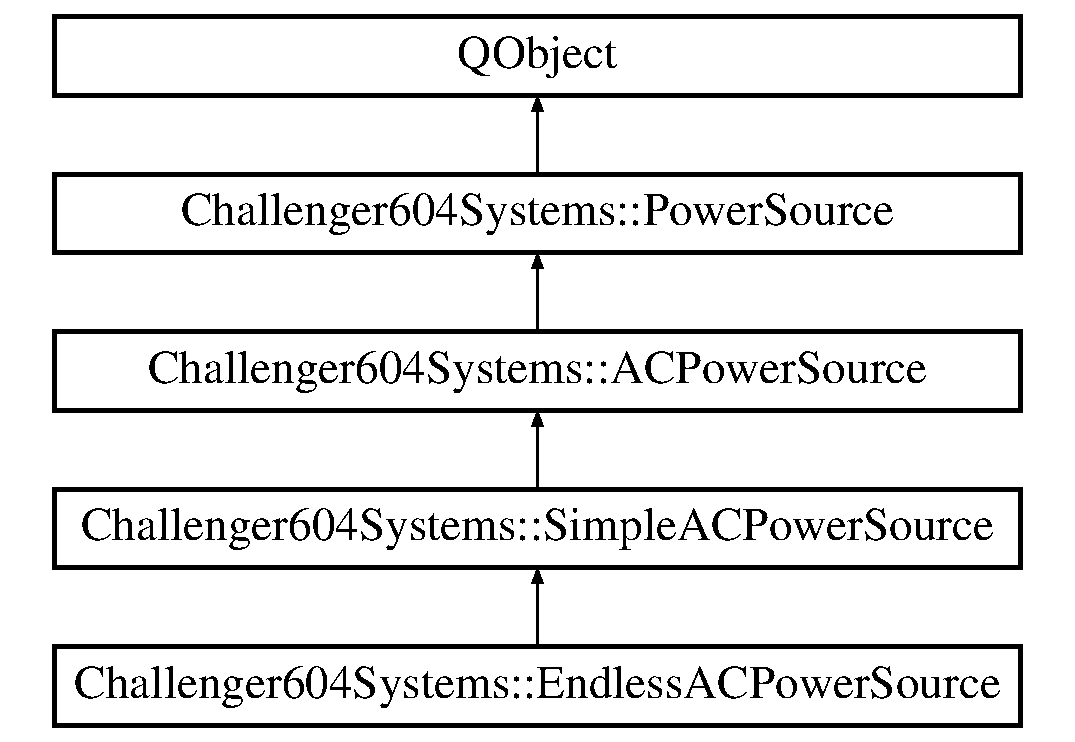
\includegraphics[height=4.000000cm]{class_challenger604_systems_1_1_a_c_power_source}
\end{center}
\end{figure}
\subsection*{Public Member Functions}
\begin{DoxyCompactItemize}
\item 
\hypertarget{class_challenger604_systems_1_1_a_c_power_source_a6574e889b593bce74090d191df02b4dd}{{\bfseries A\-C\-Power\-Source} (Q\-Object $\ast$parent=0)}\label{class_challenger604_systems_1_1_a_c_power_source_a6574e889b593bce74090d191df02b4dd}

\item 
virtual double \hyperlink{class_challenger604_systems_1_1_a_c_power_source_a022e5462d16a445f4703add09778dce4}{get\-Current\-Frequency} ()=0
\end{DoxyCompactItemize}
\subsection*{Additional Inherited Members}


\subsection{Detailed Description}
A power source that supplies A\-C power and can provide information on the frequency of the output electricity 

\subsection{Member Function Documentation}
\hypertarget{class_challenger604_systems_1_1_a_c_power_source_a022e5462d16a445f4703add09778dce4}{\index{Challenger604\-Systems\-::\-A\-C\-Power\-Source@{Challenger604\-Systems\-::\-A\-C\-Power\-Source}!get\-Current\-Frequency@{get\-Current\-Frequency}}
\index{get\-Current\-Frequency@{get\-Current\-Frequency}!Challenger604Systems::ACPowerSource@{Challenger604\-Systems\-::\-A\-C\-Power\-Source}}
\subsubsection[{get\-Current\-Frequency}]{\setlength{\rightskip}{0pt plus 5cm}virtual double Challenger604\-Systems\-::\-A\-C\-Power\-Source\-::get\-Current\-Frequency (
\begin{DoxyParamCaption}
{}
\end{DoxyParamCaption}
)\hspace{0.3cm}{\ttfamily [pure virtual]}}}\label{class_challenger604_systems_1_1_a_c_power_source_a022e5462d16a445f4703add09778dce4}
Get the frequency, in hertz, of the electricity currently being supplied by this source 

Implemented in \hyperlink{class_challenger604_systems_1_1_simple_a_c_power_source_ad125522705327fe9e78234c70e1e444f}{Challenger604\-Systems\-::\-Simple\-A\-C\-Power\-Source}.



The documentation for this class was generated from the following files\-:\begin{DoxyCompactItemize}
\item 
/\-Applications/\-X-\/\-Plane 10 Demo/\-Aircraft/\-Heavy Metal/\-Challenger 604/\-Challenger604\-Logic/electrical/defs/acpowersource.\-h\item 
/\-Applications/\-X-\/\-Plane 10 Demo/\-Aircraft/\-Heavy Metal/\-Challenger 604/\-Challenger604\-Logic/electrical/defs/acpowersource.\-cpp\end{DoxyCompactItemize}

\hypertarget{class_challenger604_systems_1_1_a_p_u}{\section{Challenger604\-Systems\-:\-:A\-P\-U Class Reference}
\label{class_challenger604_systems_1_1_a_p_u}\index{Challenger604\-Systems\-::\-A\-P\-U@{Challenger604\-Systems\-::\-A\-P\-U}}
}
Inheritance diagram for Challenger604\-Systems\-:\-:A\-P\-U\-:\begin{figure}[H]
\begin{center}
\leavevmode
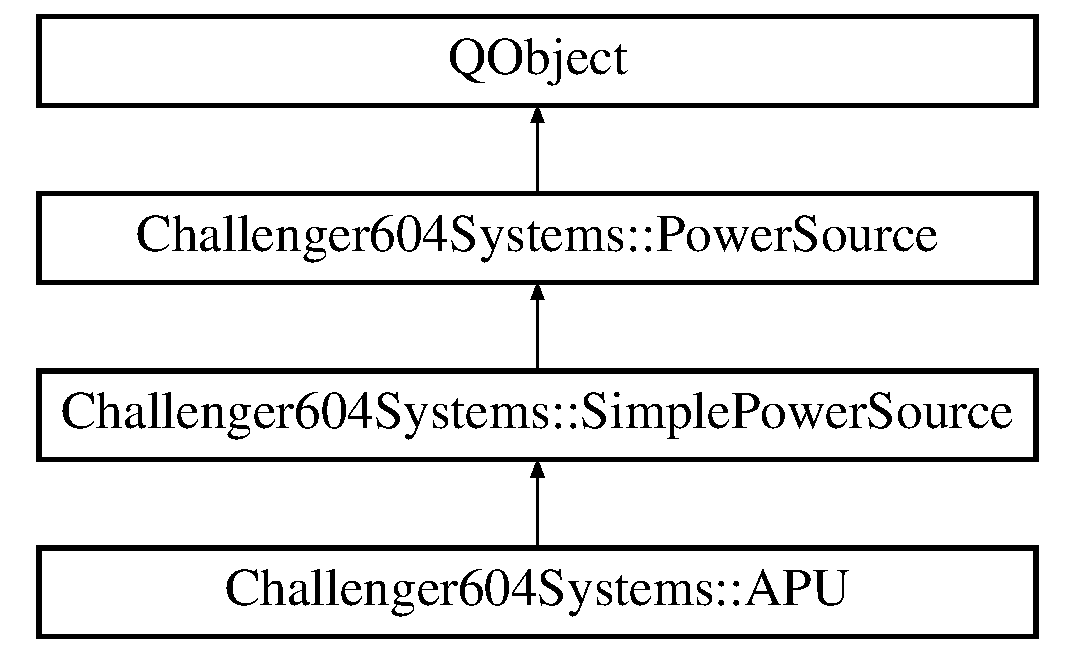
\includegraphics[height=4.000000cm]{class_challenger604_systems_1_1_a_p_u}
\end{center}
\end{figure}
\subsection*{Public Member Functions}
\begin{DoxyCompactItemize}
\item 
\hypertarget{class_challenger604_systems_1_1_a_p_u_aaa90feec507ea4f9b5eff275d2f040da}{{\bfseries A\-P\-U} (Q\-Object $\ast$parent=0)}\label{class_challenger604_systems_1_1_a_p_u_aaa90feec507ea4f9b5eff275d2f040da}

\end{DoxyCompactItemize}
\subsection*{Additional Inherited Members}


The documentation for this class was generated from the following files\-:\begin{DoxyCompactItemize}
\item 
/\-Applications/\-X-\/\-Plane 10 Demo/\-Aircraft/\-Heavy Metal/\-Challenger 604/\-Challenger604\-Logic/apu.\-h\item 
/\-Applications/\-X-\/\-Plane 10 Demo/\-Aircraft/\-Heavy Metal/\-Challenger 604/\-Challenger604\-Logic/apu.\-cpp\end{DoxyCompactItemize}

\hypertarget{class_challenger604_systems_1_1_power_source}{\section{Challenger604\-Systems\-:\-:Power\-Source Class Reference}
\label{class_challenger604_systems_1_1_power_source}\index{Challenger604\-Systems\-::\-Power\-Source@{Challenger604\-Systems\-::\-Power\-Source}}
}


{\ttfamily \#include $<$powersource.\-h$>$}

Inheritance diagram for Challenger604\-Systems\-:\-:Power\-Source\-:\begin{figure}[H]
\begin{center}
\leavevmode
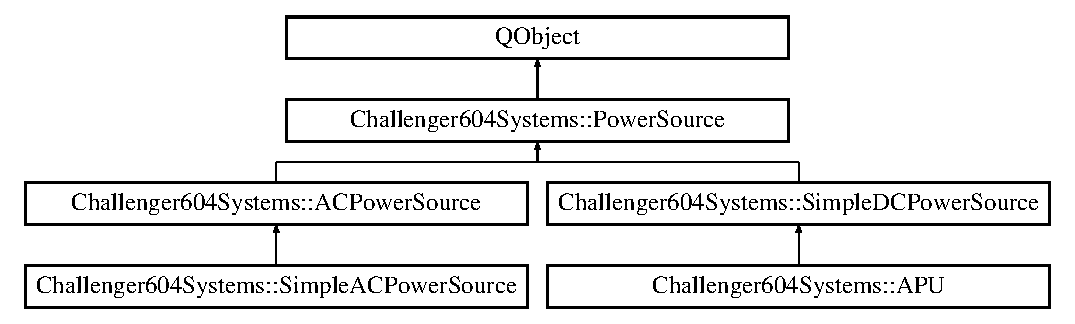
\includegraphics[height=3.174603cm]{class_challenger604_systems_1_1_power_source}
\end{center}
\end{figure}
\subsection*{Public Slots}
\begin{DoxyCompactItemize}
\item 
virtual void \hyperlink{class_challenger604_systems_1_1_power_source_a7337c7de30e3d23c551d3a41370b34bb}{request\-Power} (double in\-Requested\-Power)=0
\end{DoxyCompactItemize}
\subsection*{Public Member Functions}
\begin{DoxyCompactItemize}
\item 
\hypertarget{class_challenger604_systems_1_1_power_source_a928bccc7b0f2533f4de701926747d910}{{\bfseries Power\-Source} (Q\-Object $\ast$parent=0)}\label{class_challenger604_systems_1_1_power_source_a928bccc7b0f2533f4de701926747d910}

\item 
virtual double \hyperlink{class_challenger604_systems_1_1_power_source_a7169f0c8fdce00d38a64b6b6bba04e18}{get\-Max\-Output\-Wattage} ()=0
\item 
virtual double \hyperlink{class_challenger604_systems_1_1_power_source_afbae38476468ff99c6f0da852133d732}{get\-Available\-Output\-Wattage} ()=0
\item 
virtual double \hyperlink{class_challenger604_systems_1_1_power_source_a941b5d3a7d51811809a22126f9b16f3d}{get\-Current\-Output\-Wattage} ()=0
\item 
virtual double \hyperlink{class_challenger604_systems_1_1_power_source_a4ad8976f2c13113c87180257df806317}{get\-Current\-Output\-Voltage} ()=0
\item 
virtual \hyperlink{namespace_challenger604_systems_a9ad1a793d94b97514092692cb7315afd}{Electrical\-Power\-Type} \hyperlink{class_challenger604_systems_1_1_power_source_a005b9cac72b89344aded232d87fde2f6}{get\-Output\-Power\-Type} ()=0
\end{DoxyCompactItemize}


\subsection{Detailed Description}
An abstract class for something that can provide power to the electrical system 

\subsection{Member Function Documentation}
\hypertarget{class_challenger604_systems_1_1_power_source_afbae38476468ff99c6f0da852133d732}{\index{Challenger604\-Systems\-::\-Power\-Source@{Challenger604\-Systems\-::\-Power\-Source}!get\-Available\-Output\-Wattage@{get\-Available\-Output\-Wattage}}
\index{get\-Available\-Output\-Wattage@{get\-Available\-Output\-Wattage}!Challenger604Systems::PowerSource@{Challenger604\-Systems\-::\-Power\-Source}}
\subsubsection[{get\-Available\-Output\-Wattage}]{\setlength{\rightskip}{0pt plus 5cm}virtual double Challenger604\-Systems\-::\-Power\-Source\-::get\-Available\-Output\-Wattage (
\begin{DoxyParamCaption}
{}
\end{DoxyParamCaption}
)\hspace{0.3cm}{\ttfamily [pure virtual]}}}\label{class_challenger604_systems_1_1_power_source_afbae38476468ff99c6f0da852133d732}
Get the maximum power, in watts, that this source can provide in its current state. You may ask this device to change its state to supply more power than this by requesting a power level that is greater than this but less than the maximum power. 

Implemented in \hyperlink{class_challenger604_systems_1_1_simple_a_c_power_source_ab5c1cacdf81531a9bb73edebda3d5c0c}{Challenger604\-Systems\-::\-Simple\-A\-C\-Power\-Source}, and \hyperlink{class_challenger604_systems_1_1_simple_d_c_power_source_adb43f9aa9dba70e75d2fab1efcafc98f}{Challenger604\-Systems\-::\-Simple\-D\-C\-Power\-Source}.

\hypertarget{class_challenger604_systems_1_1_power_source_a4ad8976f2c13113c87180257df806317}{\index{Challenger604\-Systems\-::\-Power\-Source@{Challenger604\-Systems\-::\-Power\-Source}!get\-Current\-Output\-Voltage@{get\-Current\-Output\-Voltage}}
\index{get\-Current\-Output\-Voltage@{get\-Current\-Output\-Voltage}!Challenger604Systems::PowerSource@{Challenger604\-Systems\-::\-Power\-Source}}
\subsubsection[{get\-Current\-Output\-Voltage}]{\setlength{\rightskip}{0pt plus 5cm}virtual double Challenger604\-Systems\-::\-Power\-Source\-::get\-Current\-Output\-Voltage (
\begin{DoxyParamCaption}
{}
\end{DoxyParamCaption}
)\hspace{0.3cm}{\ttfamily [pure virtual]}}}\label{class_challenger604_systems_1_1_power_source_a4ad8976f2c13113c87180257df806317}
Get the voltage, in volts, of the electricity that this source is providing. 

Implemented in \hyperlink{class_challenger604_systems_1_1_simple_a_c_power_source_a1f88d86aa2bc795732a6a4d3c583ce2b}{Challenger604\-Systems\-::\-Simple\-A\-C\-Power\-Source}, and \hyperlink{class_challenger604_systems_1_1_simple_d_c_power_source_a744f905531f1876b3d66200d78e0ba56}{Challenger604\-Systems\-::\-Simple\-D\-C\-Power\-Source}.

\hypertarget{class_challenger604_systems_1_1_power_source_a941b5d3a7d51811809a22126f9b16f3d}{\index{Challenger604\-Systems\-::\-Power\-Source@{Challenger604\-Systems\-::\-Power\-Source}!get\-Current\-Output\-Wattage@{get\-Current\-Output\-Wattage}}
\index{get\-Current\-Output\-Wattage@{get\-Current\-Output\-Wattage}!Challenger604Systems::PowerSource@{Challenger604\-Systems\-::\-Power\-Source}}
\subsubsection[{get\-Current\-Output\-Wattage}]{\setlength{\rightskip}{0pt plus 5cm}virtual double Challenger604\-Systems\-::\-Power\-Source\-::get\-Current\-Output\-Wattage (
\begin{DoxyParamCaption}
{}
\end{DoxyParamCaption}
)\hspace{0.3cm}{\ttfamily [pure virtual]}}}\label{class_challenger604_systems_1_1_power_source_a941b5d3a7d51811809a22126f9b16f3d}
Get the current power, in watts, that this source is providing. This may be less than the maximum power. 

Implemented in \hyperlink{class_challenger604_systems_1_1_simple_a_c_power_source_a4e4755ba334156bf6db48e2d53b189d6}{Challenger604\-Systems\-::\-Simple\-A\-C\-Power\-Source}, and \hyperlink{class_challenger604_systems_1_1_simple_d_c_power_source_a6e35b8636ae955ce4b46f14e3b864650}{Challenger604\-Systems\-::\-Simple\-D\-C\-Power\-Source}.

\hypertarget{class_challenger604_systems_1_1_power_source_a7169f0c8fdce00d38a64b6b6bba04e18}{\index{Challenger604\-Systems\-::\-Power\-Source@{Challenger604\-Systems\-::\-Power\-Source}!get\-Max\-Output\-Wattage@{get\-Max\-Output\-Wattage}}
\index{get\-Max\-Output\-Wattage@{get\-Max\-Output\-Wattage}!Challenger604Systems::PowerSource@{Challenger604\-Systems\-::\-Power\-Source}}
\subsubsection[{get\-Max\-Output\-Wattage}]{\setlength{\rightskip}{0pt plus 5cm}virtual double Challenger604\-Systems\-::\-Power\-Source\-::get\-Max\-Output\-Wattage (
\begin{DoxyParamCaption}
{}
\end{DoxyParamCaption}
)\hspace{0.3cm}{\ttfamily [pure virtual]}}}\label{class_challenger604_systems_1_1_power_source_a7169f0c8fdce00d38a64b6b6bba04e18}
Get the maximum power, in watts, that this source can provide in any situation. 

Implemented in \hyperlink{class_challenger604_systems_1_1_simple_a_c_power_source_af4be658550a6883664eacd3ec5f63068}{Challenger604\-Systems\-::\-Simple\-A\-C\-Power\-Source}, and \hyperlink{class_challenger604_systems_1_1_simple_d_c_power_source_a9cdf826d67e23a54371a6d7840fd5ff9}{Challenger604\-Systems\-::\-Simple\-D\-C\-Power\-Source}.

\hypertarget{class_challenger604_systems_1_1_power_source_a005b9cac72b89344aded232d87fde2f6}{\index{Challenger604\-Systems\-::\-Power\-Source@{Challenger604\-Systems\-::\-Power\-Source}!get\-Output\-Power\-Type@{get\-Output\-Power\-Type}}
\index{get\-Output\-Power\-Type@{get\-Output\-Power\-Type}!Challenger604Systems::PowerSource@{Challenger604\-Systems\-::\-Power\-Source}}
\subsubsection[{get\-Output\-Power\-Type}]{\setlength{\rightskip}{0pt plus 5cm}virtual {\bf Electrical\-Power\-Type} Challenger604\-Systems\-::\-Power\-Source\-::get\-Output\-Power\-Type (
\begin{DoxyParamCaption}
{}
\end{DoxyParamCaption}
)\hspace{0.3cm}{\ttfamily [pure virtual]}}}\label{class_challenger604_systems_1_1_power_source_a005b9cac72b89344aded232d87fde2f6}
Get the type of power that this source provides 

Implemented in \hyperlink{class_challenger604_systems_1_1_simple_a_c_power_source_aaaebd8199288938f6d7955743669193b}{Challenger604\-Systems\-::\-Simple\-A\-C\-Power\-Source}, and \hyperlink{class_challenger604_systems_1_1_simple_d_c_power_source_a9253b83cb9e35b40db473e24bf3d7f54}{Challenger604\-Systems\-::\-Simple\-D\-C\-Power\-Source}.

\hypertarget{class_challenger604_systems_1_1_power_source_a7337c7de30e3d23c551d3a41370b34bb}{\index{Challenger604\-Systems\-::\-Power\-Source@{Challenger604\-Systems\-::\-Power\-Source}!request\-Power@{request\-Power}}
\index{request\-Power@{request\-Power}!Challenger604Systems::PowerSource@{Challenger604\-Systems\-::\-Power\-Source}}
\subsubsection[{request\-Power}]{\setlength{\rightskip}{0pt plus 5cm}virtual void Challenger604\-Systems\-::\-Power\-Source\-::request\-Power (
\begin{DoxyParamCaption}
\item[{double}]{in\-Requested\-Power}
\end{DoxyParamCaption}
)\hspace{0.3cm}{\ttfamily [pure virtual]}, {\ttfamily [slot]}}}\label{class_challenger604_systems_1_1_power_source_a7337c7de30e3d23c551d3a41370b34bb}
Ask this power source to provide power 
\begin{DoxyParams}{Parameters}
{\em in\-Requested\-Power} & The power, in watts, that this power source is requested to supply. If this is greater than the maximum power level, the source will supply its maximum power level.\\
\hline
\end{DoxyParams}
The source may not immediately make the requested power level available. It may take some time to \char`\"{}warm up\char`\"{}. 

The documentation for this class was generated from the following files\-:\begin{DoxyCompactItemize}
\item 
/\-Applications/\-X-\/\-Plane 10 Demo/\-Aircraft/\-Heavy Metal/\-Challenger 604/\-Challenger604\-Logic/electrical/defs/powersource.\-h\item 
/\-Applications/\-X-\/\-Plane 10 Demo/\-Aircraft/\-Heavy Metal/\-Challenger 604/\-Challenger604\-Logic/electrical/defs/powersource.\-cpp\end{DoxyCompactItemize}

\hypertarget{class_challenger604_systems_1_1_simple_a_c_power_source}{\section{Challenger604\-Systems\-:\-:Simple\-A\-C\-Power\-Source Class Reference}
\label{class_challenger604_systems_1_1_simple_a_c_power_source}\index{Challenger604\-Systems\-::\-Simple\-A\-C\-Power\-Source@{Challenger604\-Systems\-::\-Simple\-A\-C\-Power\-Source}}
}


{\ttfamily \#include $<$simpleacpowersource.\-h$>$}

Inheritance diagram for Challenger604\-Systems\-:\-:Simple\-A\-C\-Power\-Source\-:\begin{figure}[H]
\begin{center}
\leavevmode
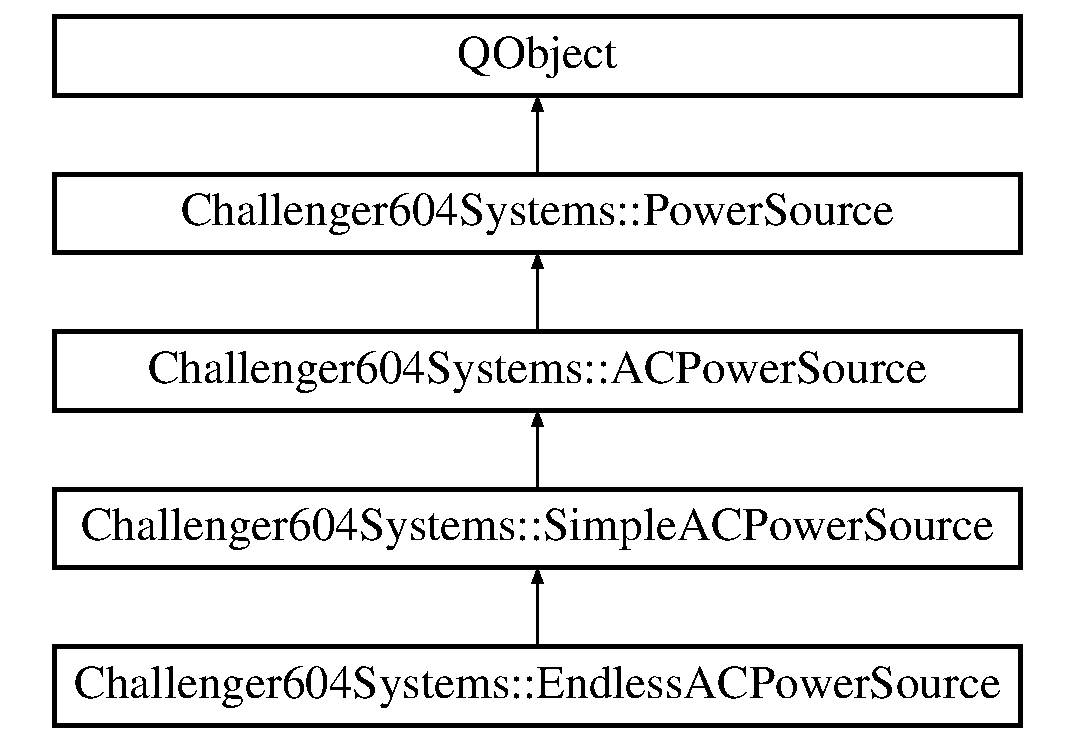
\includegraphics[height=5.000000cm]{class_challenger604_systems_1_1_simple_a_c_power_source}
\end{center}
\end{figure}
\subsection*{Public Slots}
\begin{DoxyCompactItemize}
\item 
\hypertarget{class_challenger604_systems_1_1_simple_a_c_power_source_a9f35b05f8a01cd0baa2d6de5fc1df083}{virtual void {\bfseries request\-Power} (double in\-Requested\-Power)}\label{class_challenger604_systems_1_1_simple_a_c_power_source_a9f35b05f8a01cd0baa2d6de5fc1df083}

\end{DoxyCompactItemize}
\subsection*{Public Member Functions}
\begin{DoxyCompactItemize}
\item 
\hypertarget{class_challenger604_systems_1_1_simple_a_c_power_source_afb2f7b55ab007667b09d338c17f477ed}{{\bfseries Simple\-A\-C\-Power\-Source} (Q\-Object $\ast$parent=0)}\label{class_challenger604_systems_1_1_simple_a_c_power_source_afb2f7b55ab007667b09d338c17f477ed}

\item 
virtual double \hyperlink{class_challenger604_systems_1_1_simple_a_c_power_source_ae330676157035c37441d3c8bfc198c2e}{get\-Max\-Wattage} ()
\item 
virtual double \hyperlink{class_challenger604_systems_1_1_simple_a_c_power_source_ac20e3e1da3458450951998370cd57601}{get\-Available\-Wattage} ()
\item 
virtual double \hyperlink{class_challenger604_systems_1_1_simple_a_c_power_source_a151696a75ded62c4df93b8597a5a0c2a}{get\-Current\-Wattage} ()
\item 
virtual double \hyperlink{class_challenger604_systems_1_1_simple_a_c_power_source_a04f64b1611005171ebb491b84508bcc7}{get\-Current\-Voltage} ()
\item 
virtual double \hyperlink{class_challenger604_systems_1_1_simple_a_c_power_source_ad125522705327fe9e78234c70e1e444f}{get\-Current\-Frequency} ()
\item 
virtual \hyperlink{namespace_challenger604_systems_a9ad1a793d94b97514092692cb7315afd}{Electrical\-Power\-Type} \hyperlink{class_challenger604_systems_1_1_simple_a_c_power_source_aaaebd8199288938f6d7955743669193b}{get\-Output\-Power\-Type} ()
\end{DoxyCompactItemize}
\subsection*{Protected Attributes}
\begin{DoxyCompactItemize}
\item 
double \hyperlink{class_challenger604_systems_1_1_simple_a_c_power_source_a52f945e3cf2a2ece8a3d9f772d5cddce}{max\-Wattage}
\item 
double \hyperlink{class_challenger604_systems_1_1_simple_a_c_power_source_af9aab8bb1f32a240aba9b6c4ac969ba9}{available\-Wattage}
\item 
double \hyperlink{class_challenger604_systems_1_1_simple_a_c_power_source_a555e44c4500e6f094e9fb7ca17939648}{current\-Wattage}
\item 
double \hyperlink{class_challenger604_systems_1_1_simple_a_c_power_source_aeae97501266decbd321fe2a934d5f225}{requested\-Power}
\item 
double \hyperlink{class_challenger604_systems_1_1_simple_a_c_power_source_a10506cd4ead6a716f150baaaa4c56888}{current\-Voltage}
\item 
double \hyperlink{class_challenger604_systems_1_1_simple_a_c_power_source_a321cb77fea6e9d7a79fd69d2bd7a7227}{current\-Frequency}
\end{DoxyCompactItemize}


\subsection{Detailed Description}
Extends \hyperlink{class_challenger604_systems_1_1_power_source}{Power\-Source} with built-\/in fields for maximum, available, current, and requested power levels as well as voltage and A\-C frequency. This is useful for power sources that don't have to do complicated things with their power levels. This supplies A\-C electricity at nominal 115 volts/400 hertz. All these functions are virtual, so you can override them. 

\subsection{Member Function Documentation}
\hypertarget{class_challenger604_systems_1_1_simple_a_c_power_source_ac20e3e1da3458450951998370cd57601}{\index{Challenger604\-Systems\-::\-Simple\-A\-C\-Power\-Source@{Challenger604\-Systems\-::\-Simple\-A\-C\-Power\-Source}!get\-Available\-Wattage@{get\-Available\-Wattage}}
\index{get\-Available\-Wattage@{get\-Available\-Wattage}!Challenger604Systems::SimpleACPowerSource@{Challenger604\-Systems\-::\-Simple\-A\-C\-Power\-Source}}
\subsubsection[{get\-Available\-Wattage}]{\setlength{\rightskip}{0pt plus 5cm}double Challenger604\-Systems\-::\-Simple\-A\-C\-Power\-Source\-::get\-Available\-Wattage (
\begin{DoxyParamCaption}
{}
\end{DoxyParamCaption}
)\hspace{0.3cm}{\ttfamily [virtual]}}}\label{class_challenger604_systems_1_1_simple_a_c_power_source_ac20e3e1da3458450951998370cd57601}
Get the maximum power, in watts, that this source can provide in its current state. You may ask this device to change its state to supply more power than this by requesting a power level that is greater than this but less than the maximum power. 

Implements \hyperlink{class_challenger604_systems_1_1_power_source_a35af892773c7a60f4d6ac031755cd104}{Challenger604\-Systems\-::\-Power\-Source}.

\hypertarget{class_challenger604_systems_1_1_simple_a_c_power_source_ad125522705327fe9e78234c70e1e444f}{\index{Challenger604\-Systems\-::\-Simple\-A\-C\-Power\-Source@{Challenger604\-Systems\-::\-Simple\-A\-C\-Power\-Source}!get\-Current\-Frequency@{get\-Current\-Frequency}}
\index{get\-Current\-Frequency@{get\-Current\-Frequency}!Challenger604Systems::SimpleACPowerSource@{Challenger604\-Systems\-::\-Simple\-A\-C\-Power\-Source}}
\subsubsection[{get\-Current\-Frequency}]{\setlength{\rightskip}{0pt plus 5cm}double Challenger604\-Systems\-::\-Simple\-A\-C\-Power\-Source\-::get\-Current\-Frequency (
\begin{DoxyParamCaption}
{}
\end{DoxyParamCaption}
)\hspace{0.3cm}{\ttfamily [virtual]}}}\label{class_challenger604_systems_1_1_simple_a_c_power_source_ad125522705327fe9e78234c70e1e444f}
Get the frequency, in hertz, of the electricity currently being supplied by this source 

Implements \hyperlink{class_challenger604_systems_1_1_a_c_power_source_a022e5462d16a445f4703add09778dce4}{Challenger604\-Systems\-::\-A\-C\-Power\-Source}.

\hypertarget{class_challenger604_systems_1_1_simple_a_c_power_source_a04f64b1611005171ebb491b84508bcc7}{\index{Challenger604\-Systems\-::\-Simple\-A\-C\-Power\-Source@{Challenger604\-Systems\-::\-Simple\-A\-C\-Power\-Source}!get\-Current\-Voltage@{get\-Current\-Voltage}}
\index{get\-Current\-Voltage@{get\-Current\-Voltage}!Challenger604Systems::SimpleACPowerSource@{Challenger604\-Systems\-::\-Simple\-A\-C\-Power\-Source}}
\subsubsection[{get\-Current\-Voltage}]{\setlength{\rightskip}{0pt plus 5cm}double Challenger604\-Systems\-::\-Simple\-A\-C\-Power\-Source\-::get\-Current\-Voltage (
\begin{DoxyParamCaption}
{}
\end{DoxyParamCaption}
)\hspace{0.3cm}{\ttfamily [virtual]}}}\label{class_challenger604_systems_1_1_simple_a_c_power_source_a04f64b1611005171ebb491b84508bcc7}
Get the voltage, in volts, of the electricity that this source is providing. 

Implements \hyperlink{class_challenger604_systems_1_1_power_source_af432be401da09206f49439f6c5299176}{Challenger604\-Systems\-::\-Power\-Source}.

\hypertarget{class_challenger604_systems_1_1_simple_a_c_power_source_a151696a75ded62c4df93b8597a5a0c2a}{\index{Challenger604\-Systems\-::\-Simple\-A\-C\-Power\-Source@{Challenger604\-Systems\-::\-Simple\-A\-C\-Power\-Source}!get\-Current\-Wattage@{get\-Current\-Wattage}}
\index{get\-Current\-Wattage@{get\-Current\-Wattage}!Challenger604Systems::SimpleACPowerSource@{Challenger604\-Systems\-::\-Simple\-A\-C\-Power\-Source}}
\subsubsection[{get\-Current\-Wattage}]{\setlength{\rightskip}{0pt plus 5cm}double Challenger604\-Systems\-::\-Simple\-A\-C\-Power\-Source\-::get\-Current\-Wattage (
\begin{DoxyParamCaption}
{}
\end{DoxyParamCaption}
)\hspace{0.3cm}{\ttfamily [virtual]}}}\label{class_challenger604_systems_1_1_simple_a_c_power_source_a151696a75ded62c4df93b8597a5a0c2a}
Get the current power, in watts, that this source is providing. This may be less than the maximum power. 

Implements \hyperlink{class_challenger604_systems_1_1_power_source_a82252be3f4e80239848bd9cadb69ec31}{Challenger604\-Systems\-::\-Power\-Source}.

\hypertarget{class_challenger604_systems_1_1_simple_a_c_power_source_ae330676157035c37441d3c8bfc198c2e}{\index{Challenger604\-Systems\-::\-Simple\-A\-C\-Power\-Source@{Challenger604\-Systems\-::\-Simple\-A\-C\-Power\-Source}!get\-Max\-Wattage@{get\-Max\-Wattage}}
\index{get\-Max\-Wattage@{get\-Max\-Wattage}!Challenger604Systems::SimpleACPowerSource@{Challenger604\-Systems\-::\-Simple\-A\-C\-Power\-Source}}
\subsubsection[{get\-Max\-Wattage}]{\setlength{\rightskip}{0pt plus 5cm}double Challenger604\-Systems\-::\-Simple\-A\-C\-Power\-Source\-::get\-Max\-Wattage (
\begin{DoxyParamCaption}
{}
\end{DoxyParamCaption}
)\hspace{0.3cm}{\ttfamily [virtual]}}}\label{class_challenger604_systems_1_1_simple_a_c_power_source_ae330676157035c37441d3c8bfc198c2e}
Get the maximum power, in watts, that this source can provide in any situation. 

Implements \hyperlink{class_challenger604_systems_1_1_power_source_aed53a668295c22fabdf8adf8018d8d1d}{Challenger604\-Systems\-::\-Power\-Source}.

\hypertarget{class_challenger604_systems_1_1_simple_a_c_power_source_aaaebd8199288938f6d7955743669193b}{\index{Challenger604\-Systems\-::\-Simple\-A\-C\-Power\-Source@{Challenger604\-Systems\-::\-Simple\-A\-C\-Power\-Source}!get\-Output\-Power\-Type@{get\-Output\-Power\-Type}}
\index{get\-Output\-Power\-Type@{get\-Output\-Power\-Type}!Challenger604Systems::SimpleACPowerSource@{Challenger604\-Systems\-::\-Simple\-A\-C\-Power\-Source}}
\subsubsection[{get\-Output\-Power\-Type}]{\setlength{\rightskip}{0pt plus 5cm}{\bf Electrical\-Power\-Type} Challenger604\-Systems\-::\-Simple\-A\-C\-Power\-Source\-::get\-Output\-Power\-Type (
\begin{DoxyParamCaption}
{}
\end{DoxyParamCaption}
)\hspace{0.3cm}{\ttfamily [virtual]}}}\label{class_challenger604_systems_1_1_simple_a_c_power_source_aaaebd8199288938f6d7955743669193b}
Get the type of power that this source provides 

Implements \hyperlink{class_challenger604_systems_1_1_power_source_a005b9cac72b89344aded232d87fde2f6}{Challenger604\-Systems\-::\-Power\-Source}.



\subsection{Member Data Documentation}
\hypertarget{class_challenger604_systems_1_1_simple_a_c_power_source_af9aab8bb1f32a240aba9b6c4ac969ba9}{\index{Challenger604\-Systems\-::\-Simple\-A\-C\-Power\-Source@{Challenger604\-Systems\-::\-Simple\-A\-C\-Power\-Source}!available\-Wattage@{available\-Wattage}}
\index{available\-Wattage@{available\-Wattage}!Challenger604Systems::SimpleACPowerSource@{Challenger604\-Systems\-::\-Simple\-A\-C\-Power\-Source}}
\subsubsection[{available\-Wattage}]{\setlength{\rightskip}{0pt plus 5cm}double Challenger604\-Systems\-::\-Simple\-A\-C\-Power\-Source\-::available\-Wattage\hspace{0.3cm}{\ttfamily [protected]}}}\label{class_challenger604_systems_1_1_simple_a_c_power_source_af9aab8bb1f32a240aba9b6c4ac969ba9}
The maximum power that this source can supply in its current state \hypertarget{class_challenger604_systems_1_1_simple_a_c_power_source_a321cb77fea6e9d7a79fd69d2bd7a7227}{\index{Challenger604\-Systems\-::\-Simple\-A\-C\-Power\-Source@{Challenger604\-Systems\-::\-Simple\-A\-C\-Power\-Source}!current\-Frequency@{current\-Frequency}}
\index{current\-Frequency@{current\-Frequency}!Challenger604Systems::SimpleACPowerSource@{Challenger604\-Systems\-::\-Simple\-A\-C\-Power\-Source}}
\subsubsection[{current\-Frequency}]{\setlength{\rightskip}{0pt plus 5cm}double Challenger604\-Systems\-::\-Simple\-A\-C\-Power\-Source\-::current\-Frequency\hspace{0.3cm}{\ttfamily [protected]}}}\label{class_challenger604_systems_1_1_simple_a_c_power_source_a321cb77fea6e9d7a79fd69d2bd7a7227}
The frequency of the electricity that is currently being supplied \hypertarget{class_challenger604_systems_1_1_simple_a_c_power_source_a10506cd4ead6a716f150baaaa4c56888}{\index{Challenger604\-Systems\-::\-Simple\-A\-C\-Power\-Source@{Challenger604\-Systems\-::\-Simple\-A\-C\-Power\-Source}!current\-Voltage@{current\-Voltage}}
\index{current\-Voltage@{current\-Voltage}!Challenger604Systems::SimpleACPowerSource@{Challenger604\-Systems\-::\-Simple\-A\-C\-Power\-Source}}
\subsubsection[{current\-Voltage}]{\setlength{\rightskip}{0pt plus 5cm}double Challenger604\-Systems\-::\-Simple\-A\-C\-Power\-Source\-::current\-Voltage\hspace{0.3cm}{\ttfamily [protected]}}}\label{class_challenger604_systems_1_1_simple_a_c_power_source_a10506cd4ead6a716f150baaaa4c56888}
The voltage that is currently being supplied \hypertarget{class_challenger604_systems_1_1_simple_a_c_power_source_a555e44c4500e6f094e9fb7ca17939648}{\index{Challenger604\-Systems\-::\-Simple\-A\-C\-Power\-Source@{Challenger604\-Systems\-::\-Simple\-A\-C\-Power\-Source}!current\-Wattage@{current\-Wattage}}
\index{current\-Wattage@{current\-Wattage}!Challenger604Systems::SimpleACPowerSource@{Challenger604\-Systems\-::\-Simple\-A\-C\-Power\-Source}}
\subsubsection[{current\-Wattage}]{\setlength{\rightskip}{0pt plus 5cm}double Challenger604\-Systems\-::\-Simple\-A\-C\-Power\-Source\-::current\-Wattage\hspace{0.3cm}{\ttfamily [protected]}}}\label{class_challenger604_systems_1_1_simple_a_c_power_source_a555e44c4500e6f094e9fb7ca17939648}
The current power that this source is supplying \hypertarget{class_challenger604_systems_1_1_simple_a_c_power_source_a52f945e3cf2a2ece8a3d9f772d5cddce}{\index{Challenger604\-Systems\-::\-Simple\-A\-C\-Power\-Source@{Challenger604\-Systems\-::\-Simple\-A\-C\-Power\-Source}!max\-Wattage@{max\-Wattage}}
\index{max\-Wattage@{max\-Wattage}!Challenger604Systems::SimpleACPowerSource@{Challenger604\-Systems\-::\-Simple\-A\-C\-Power\-Source}}
\subsubsection[{max\-Wattage}]{\setlength{\rightskip}{0pt plus 5cm}double Challenger604\-Systems\-::\-Simple\-A\-C\-Power\-Source\-::max\-Wattage\hspace{0.3cm}{\ttfamily [protected]}}}\label{class_challenger604_systems_1_1_simple_a_c_power_source_a52f945e3cf2a2ece8a3d9f772d5cddce}
The maximum power that this source can supply \hypertarget{class_challenger604_systems_1_1_simple_a_c_power_source_aeae97501266decbd321fe2a934d5f225}{\index{Challenger604\-Systems\-::\-Simple\-A\-C\-Power\-Source@{Challenger604\-Systems\-::\-Simple\-A\-C\-Power\-Source}!requested\-Power@{requested\-Power}}
\index{requested\-Power@{requested\-Power}!Challenger604Systems::SimpleACPowerSource@{Challenger604\-Systems\-::\-Simple\-A\-C\-Power\-Source}}
\subsubsection[{requested\-Power}]{\setlength{\rightskip}{0pt plus 5cm}double Challenger604\-Systems\-::\-Simple\-A\-C\-Power\-Source\-::requested\-Power\hspace{0.3cm}{\ttfamily [protected]}}}\label{class_challenger604_systems_1_1_simple_a_c_power_source_aeae97501266decbd321fe2a934d5f225}
The power that is currently requested 

The documentation for this class was generated from the following files\-:\begin{DoxyCompactItemize}
\item 
/\-Applications/\-X-\/\-Plane 10 Demo/\-Aircraft/\-Heavy Metal/\-Challenger 604/\-Challenger604\-Logic/electrical/defs/simpleacpowersource.\-h\item 
/\-Applications/\-X-\/\-Plane 10 Demo/\-Aircraft/\-Heavy Metal/\-Challenger 604/\-Challenger604\-Logic/electrical/defs/simpleacpowersource.\-cpp\end{DoxyCompactItemize}

\hypertarget{class_challenger604_systems_1_1_simple_d_c_power_source}{\section{Challenger604\-Systems\-:\-:Simple\-D\-C\-Power\-Source Class Reference}
\label{class_challenger604_systems_1_1_simple_d_c_power_source}\index{Challenger604\-Systems\-::\-Simple\-D\-C\-Power\-Source@{Challenger604\-Systems\-::\-Simple\-D\-C\-Power\-Source}}
}


{\ttfamily \#include $<$simpledcpowersource.\-h$>$}

Inheritance diagram for Challenger604\-Systems\-:\-:Simple\-D\-C\-Power\-Source\-:\begin{figure}[H]
\begin{center}
\leavevmode
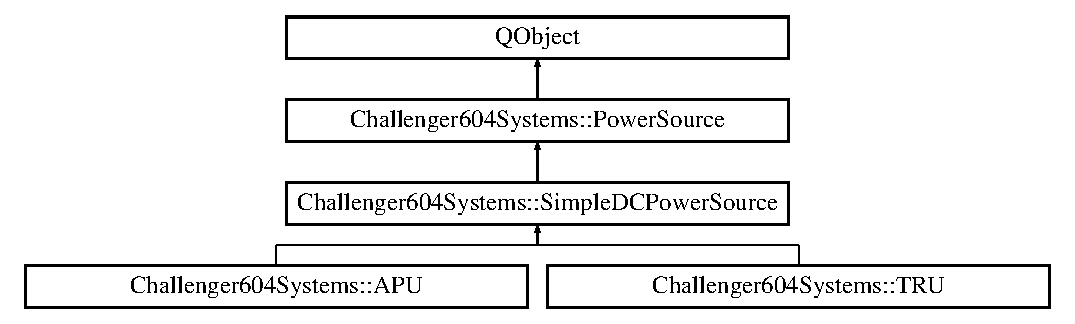
\includegraphics[height=3.902439cm]{class_challenger604_systems_1_1_simple_d_c_power_source}
\end{center}
\end{figure}
\subsection*{Public Slots}
\begin{DoxyCompactItemize}
\item 
\hypertarget{class_challenger604_systems_1_1_simple_d_c_power_source_a7af4e82286499ec04189398fa14b7b9f}{virtual void {\bfseries request\-Power} (double in\-Requested\-Power)}\label{class_challenger604_systems_1_1_simple_d_c_power_source_a7af4e82286499ec04189398fa14b7b9f}

\end{DoxyCompactItemize}
\subsection*{Public Member Functions}
\begin{DoxyCompactItemize}
\item 
\hypertarget{class_challenger604_systems_1_1_simple_d_c_power_source_a874e451053b69d48b2bbdf924ce05dde}{{\bfseries Simple\-D\-C\-Power\-Source} (Q\-Object $\ast$parent=0)}\label{class_challenger604_systems_1_1_simple_d_c_power_source_a874e451053b69d48b2bbdf924ce05dde}

\item 
virtual double \hyperlink{class_challenger604_systems_1_1_simple_d_c_power_source_ad6285e377af915c21bf15637732f0291}{get\-Max\-Wattage} ()
\item 
virtual double \hyperlink{class_challenger604_systems_1_1_simple_d_c_power_source_a47085e7418e1e327552bd4339d08621a}{get\-Available\-Wattage} ()
\item 
virtual double \hyperlink{class_challenger604_systems_1_1_simple_d_c_power_source_ac1f53b3d602f8279f3b80bf9280b62d9}{get\-Current\-Wattage} ()
\item 
virtual double \hyperlink{class_challenger604_systems_1_1_simple_d_c_power_source_a19a6be7acae4e8183a0b03f0e948f659}{get\-Current\-Voltage} ()
\item 
virtual \hyperlink{namespace_challenger604_systems_a9ad1a793d94b97514092692cb7315afd}{Electrical\-Power\-Type} \hyperlink{class_challenger604_systems_1_1_simple_d_c_power_source_a9253b83cb9e35b40db473e24bf3d7f54}{get\-Output\-Power\-Type} ()
\end{DoxyCompactItemize}
\subsection*{Protected Attributes}
\begin{DoxyCompactItemize}
\item 
double \hyperlink{class_challenger604_systems_1_1_simple_d_c_power_source_a7ccc3391b03c04b09f6792e0a44b026b}{max\-Wattage}
\item 
double \hyperlink{class_challenger604_systems_1_1_simple_d_c_power_source_a1e32a5e348dca6e2043f539a434debd9}{available\-Wattage}
\item 
double \hyperlink{class_challenger604_systems_1_1_simple_d_c_power_source_a5c8c5b89f6d3cd3d332ee12ef893839c}{current\-Wattage}
\item 
double \hyperlink{class_challenger604_systems_1_1_simple_d_c_power_source_a37f983774689318c3cb0295380ce4bd7}{requested\-Power}
\item 
double \hyperlink{class_challenger604_systems_1_1_simple_d_c_power_source_a6d5b229b66f1e6396229561e9a9562e4}{current\-Voltage}
\end{DoxyCompactItemize}


\subsection{Detailed Description}
Extends \hyperlink{class_challenger604_systems_1_1_power_source}{Power\-Source} with built-\/in fields for maximum, available, current, and requested power levels as well as voltage. This is useful for power sources that don't have to do complicated things with their power levels. This supplies D\-C electricity at nominal 28 volts. All these functions are virtual, so you can override them. 

\subsection{Member Function Documentation}
\hypertarget{class_challenger604_systems_1_1_simple_d_c_power_source_a47085e7418e1e327552bd4339d08621a}{\index{Challenger604\-Systems\-::\-Simple\-D\-C\-Power\-Source@{Challenger604\-Systems\-::\-Simple\-D\-C\-Power\-Source}!get\-Available\-Wattage@{get\-Available\-Wattage}}
\index{get\-Available\-Wattage@{get\-Available\-Wattage}!Challenger604Systems::SimpleDCPowerSource@{Challenger604\-Systems\-::\-Simple\-D\-C\-Power\-Source}}
\subsubsection[{get\-Available\-Wattage}]{\setlength{\rightskip}{0pt plus 5cm}double Challenger604\-Systems\-::\-Simple\-D\-C\-Power\-Source\-::get\-Available\-Wattage (
\begin{DoxyParamCaption}
{}
\end{DoxyParamCaption}
)\hspace{0.3cm}{\ttfamily [virtual]}}}\label{class_challenger604_systems_1_1_simple_d_c_power_source_a47085e7418e1e327552bd4339d08621a}
Get the maximum power, in watts, that this source can provide in its current state. You may ask this device to change its state to supply more power than this by requesting a power level that is greater than this but less than the maximum power. 

Implements \hyperlink{class_challenger604_systems_1_1_power_source_a35af892773c7a60f4d6ac031755cd104}{Challenger604\-Systems\-::\-Power\-Source}.

\hypertarget{class_challenger604_systems_1_1_simple_d_c_power_source_a19a6be7acae4e8183a0b03f0e948f659}{\index{Challenger604\-Systems\-::\-Simple\-D\-C\-Power\-Source@{Challenger604\-Systems\-::\-Simple\-D\-C\-Power\-Source}!get\-Current\-Voltage@{get\-Current\-Voltage}}
\index{get\-Current\-Voltage@{get\-Current\-Voltage}!Challenger604Systems::SimpleDCPowerSource@{Challenger604\-Systems\-::\-Simple\-D\-C\-Power\-Source}}
\subsubsection[{get\-Current\-Voltage}]{\setlength{\rightskip}{0pt plus 5cm}double Challenger604\-Systems\-::\-Simple\-D\-C\-Power\-Source\-::get\-Current\-Voltage (
\begin{DoxyParamCaption}
{}
\end{DoxyParamCaption}
)\hspace{0.3cm}{\ttfamily [virtual]}}}\label{class_challenger604_systems_1_1_simple_d_c_power_source_a19a6be7acae4e8183a0b03f0e948f659}
Get the voltage, in volts, of the electricity that this source is providing. 

Implements \hyperlink{class_challenger604_systems_1_1_power_source_af432be401da09206f49439f6c5299176}{Challenger604\-Systems\-::\-Power\-Source}.

\hypertarget{class_challenger604_systems_1_1_simple_d_c_power_source_ac1f53b3d602f8279f3b80bf9280b62d9}{\index{Challenger604\-Systems\-::\-Simple\-D\-C\-Power\-Source@{Challenger604\-Systems\-::\-Simple\-D\-C\-Power\-Source}!get\-Current\-Wattage@{get\-Current\-Wattage}}
\index{get\-Current\-Wattage@{get\-Current\-Wattage}!Challenger604Systems::SimpleDCPowerSource@{Challenger604\-Systems\-::\-Simple\-D\-C\-Power\-Source}}
\subsubsection[{get\-Current\-Wattage}]{\setlength{\rightskip}{0pt plus 5cm}double Challenger604\-Systems\-::\-Simple\-D\-C\-Power\-Source\-::get\-Current\-Wattage (
\begin{DoxyParamCaption}
{}
\end{DoxyParamCaption}
)\hspace{0.3cm}{\ttfamily [virtual]}}}\label{class_challenger604_systems_1_1_simple_d_c_power_source_ac1f53b3d602f8279f3b80bf9280b62d9}
Get the current power, in watts, that this source is providing. This may be less than the maximum power. 

Implements \hyperlink{class_challenger604_systems_1_1_power_source_a82252be3f4e80239848bd9cadb69ec31}{Challenger604\-Systems\-::\-Power\-Source}.

\hypertarget{class_challenger604_systems_1_1_simple_d_c_power_source_ad6285e377af915c21bf15637732f0291}{\index{Challenger604\-Systems\-::\-Simple\-D\-C\-Power\-Source@{Challenger604\-Systems\-::\-Simple\-D\-C\-Power\-Source}!get\-Max\-Wattage@{get\-Max\-Wattage}}
\index{get\-Max\-Wattage@{get\-Max\-Wattage}!Challenger604Systems::SimpleDCPowerSource@{Challenger604\-Systems\-::\-Simple\-D\-C\-Power\-Source}}
\subsubsection[{get\-Max\-Wattage}]{\setlength{\rightskip}{0pt plus 5cm}double Challenger604\-Systems\-::\-Simple\-D\-C\-Power\-Source\-::get\-Max\-Wattage (
\begin{DoxyParamCaption}
{}
\end{DoxyParamCaption}
)\hspace{0.3cm}{\ttfamily [virtual]}}}\label{class_challenger604_systems_1_1_simple_d_c_power_source_ad6285e377af915c21bf15637732f0291}
Get the maximum power, in watts, that this source can provide in any situation. 

Implements \hyperlink{class_challenger604_systems_1_1_power_source_aed53a668295c22fabdf8adf8018d8d1d}{Challenger604\-Systems\-::\-Power\-Source}.

\hypertarget{class_challenger604_systems_1_1_simple_d_c_power_source_a9253b83cb9e35b40db473e24bf3d7f54}{\index{Challenger604\-Systems\-::\-Simple\-D\-C\-Power\-Source@{Challenger604\-Systems\-::\-Simple\-D\-C\-Power\-Source}!get\-Output\-Power\-Type@{get\-Output\-Power\-Type}}
\index{get\-Output\-Power\-Type@{get\-Output\-Power\-Type}!Challenger604Systems::SimpleDCPowerSource@{Challenger604\-Systems\-::\-Simple\-D\-C\-Power\-Source}}
\subsubsection[{get\-Output\-Power\-Type}]{\setlength{\rightskip}{0pt plus 5cm}{\bf Electrical\-Power\-Type} Challenger604\-Systems\-::\-Simple\-D\-C\-Power\-Source\-::get\-Output\-Power\-Type (
\begin{DoxyParamCaption}
{}
\end{DoxyParamCaption}
)\hspace{0.3cm}{\ttfamily [virtual]}}}\label{class_challenger604_systems_1_1_simple_d_c_power_source_a9253b83cb9e35b40db473e24bf3d7f54}
Get the type of power that this source provides 

Implements \hyperlink{class_challenger604_systems_1_1_power_source_a005b9cac72b89344aded232d87fde2f6}{Challenger604\-Systems\-::\-Power\-Source}.



\subsection{Member Data Documentation}
\hypertarget{class_challenger604_systems_1_1_simple_d_c_power_source_a1e32a5e348dca6e2043f539a434debd9}{\index{Challenger604\-Systems\-::\-Simple\-D\-C\-Power\-Source@{Challenger604\-Systems\-::\-Simple\-D\-C\-Power\-Source}!available\-Wattage@{available\-Wattage}}
\index{available\-Wattage@{available\-Wattage}!Challenger604Systems::SimpleDCPowerSource@{Challenger604\-Systems\-::\-Simple\-D\-C\-Power\-Source}}
\subsubsection[{available\-Wattage}]{\setlength{\rightskip}{0pt plus 5cm}double Challenger604\-Systems\-::\-Simple\-D\-C\-Power\-Source\-::available\-Wattage\hspace{0.3cm}{\ttfamily [protected]}}}\label{class_challenger604_systems_1_1_simple_d_c_power_source_a1e32a5e348dca6e2043f539a434debd9}
The maximum power that this source can supply in its current state \hypertarget{class_challenger604_systems_1_1_simple_d_c_power_source_a6d5b229b66f1e6396229561e9a9562e4}{\index{Challenger604\-Systems\-::\-Simple\-D\-C\-Power\-Source@{Challenger604\-Systems\-::\-Simple\-D\-C\-Power\-Source}!current\-Voltage@{current\-Voltage}}
\index{current\-Voltage@{current\-Voltage}!Challenger604Systems::SimpleDCPowerSource@{Challenger604\-Systems\-::\-Simple\-D\-C\-Power\-Source}}
\subsubsection[{current\-Voltage}]{\setlength{\rightskip}{0pt plus 5cm}double Challenger604\-Systems\-::\-Simple\-D\-C\-Power\-Source\-::current\-Voltage\hspace{0.3cm}{\ttfamily [protected]}}}\label{class_challenger604_systems_1_1_simple_d_c_power_source_a6d5b229b66f1e6396229561e9a9562e4}
The voltage that is currently being supplied \hypertarget{class_challenger604_systems_1_1_simple_d_c_power_source_a5c8c5b89f6d3cd3d332ee12ef893839c}{\index{Challenger604\-Systems\-::\-Simple\-D\-C\-Power\-Source@{Challenger604\-Systems\-::\-Simple\-D\-C\-Power\-Source}!current\-Wattage@{current\-Wattage}}
\index{current\-Wattage@{current\-Wattage}!Challenger604Systems::SimpleDCPowerSource@{Challenger604\-Systems\-::\-Simple\-D\-C\-Power\-Source}}
\subsubsection[{current\-Wattage}]{\setlength{\rightskip}{0pt plus 5cm}double Challenger604\-Systems\-::\-Simple\-D\-C\-Power\-Source\-::current\-Wattage\hspace{0.3cm}{\ttfamily [protected]}}}\label{class_challenger604_systems_1_1_simple_d_c_power_source_a5c8c5b89f6d3cd3d332ee12ef893839c}
The current power that this source is supplying \hypertarget{class_challenger604_systems_1_1_simple_d_c_power_source_a7ccc3391b03c04b09f6792e0a44b026b}{\index{Challenger604\-Systems\-::\-Simple\-D\-C\-Power\-Source@{Challenger604\-Systems\-::\-Simple\-D\-C\-Power\-Source}!max\-Wattage@{max\-Wattage}}
\index{max\-Wattage@{max\-Wattage}!Challenger604Systems::SimpleDCPowerSource@{Challenger604\-Systems\-::\-Simple\-D\-C\-Power\-Source}}
\subsubsection[{max\-Wattage}]{\setlength{\rightskip}{0pt plus 5cm}double Challenger604\-Systems\-::\-Simple\-D\-C\-Power\-Source\-::max\-Wattage\hspace{0.3cm}{\ttfamily [protected]}}}\label{class_challenger604_systems_1_1_simple_d_c_power_source_a7ccc3391b03c04b09f6792e0a44b026b}
The maximum power that this source can supply \hypertarget{class_challenger604_systems_1_1_simple_d_c_power_source_a37f983774689318c3cb0295380ce4bd7}{\index{Challenger604\-Systems\-::\-Simple\-D\-C\-Power\-Source@{Challenger604\-Systems\-::\-Simple\-D\-C\-Power\-Source}!requested\-Power@{requested\-Power}}
\index{requested\-Power@{requested\-Power}!Challenger604Systems::SimpleDCPowerSource@{Challenger604\-Systems\-::\-Simple\-D\-C\-Power\-Source}}
\subsubsection[{requested\-Power}]{\setlength{\rightskip}{0pt plus 5cm}double Challenger604\-Systems\-::\-Simple\-D\-C\-Power\-Source\-::requested\-Power\hspace{0.3cm}{\ttfamily [protected]}}}\label{class_challenger604_systems_1_1_simple_d_c_power_source_a37f983774689318c3cb0295380ce4bd7}
The power that is currently requested 

The documentation for this class was generated from the following files\-:\begin{DoxyCompactItemize}
\item 
/\-Applications/\-X-\/\-Plane 10 Demo/\-Aircraft/\-Heavy Metal/\-Challenger 604/\-Challenger604\-Logic/electrical/defs/simpledcpowersource.\-h\item 
/\-Applications/\-X-\/\-Plane 10 Demo/\-Aircraft/\-Heavy Metal/\-Challenger 604/\-Challenger604\-Logic/electrical/defs/simpledcpowersource.\-cpp\end{DoxyCompactItemize}

\chapter{File Documentation}
\hypertarget{electricalpowertype_8h}{\section{/\-Applications/\-X-\/\-Plane 10 Demo/\-Aircraft/\-Heavy Metal/\-Challenger 604/\-Challenger604\-Logic/electricalpowertype.h File Reference}
\label{electricalpowertype_8h}\index{/\-Applications/\-X-\/\-Plane 10 Demo/\-Aircraft/\-Heavy Metal/\-Challenger 604/\-Challenger604\-Logic/electricalpowertype.\-h@{/\-Applications/\-X-\/\-Plane 10 Demo/\-Aircraft/\-Heavy Metal/\-Challenger 604/\-Challenger604\-Logic/electricalpowertype.\-h}}
}


Contains an enum for types of electrical power.  


\subsection*{Namespaces}
\begin{DoxyCompactItemize}
\item 
namespace \hyperlink{namespace_challenger604_systems}{Challenger604\-Systems}
\begin{DoxyCompactList}\small\item\em This namespace contains everything in this project. \end{DoxyCompactList}\end{DoxyCompactItemize}
\subsection*{Enumerations}
\begin{DoxyCompactItemize}
\item 
enum \hyperlink{namespace_challenger604_systems_a9ad1a793d94b97514092692cb7315afd}{Challenger604\-Systems\-::\-Electrical\-Power\-Type} \{ \\*
\hyperlink{namespace_challenger604_systems_a9ad1a793d94b97514092692cb7315afdac443cb4f2e9c8fb362d1b23d390680c1}{Challenger604\-Systems\-::\-D\-C\-\_\-\-O\-T\-H\-E\-R}, 
\hyperlink{namespace_challenger604_systems_a9ad1a793d94b97514092692cb7315afdaeb46efa4ea7afd565b7f41c0881a206d}{Challenger604\-Systems\-::\-D\-C\-\_\-12\-V}, 
\hyperlink{namespace_challenger604_systems_a9ad1a793d94b97514092692cb7315afdaa549263d4db7adacf1008dac6a68b21d}{Challenger604\-Systems\-::\-D\-C\-\_\-28\-V}, 
\hyperlink{namespace_challenger604_systems_a9ad1a793d94b97514092692cb7315afda2fcb938b597382142bdc684898fe8596}{Challenger604\-Systems\-::\-A\-C\-\_\-\-O\-T\-H\-E\-R}, 
\\*
\hyperlink{namespace_challenger604_systems_a9ad1a793d94b97514092692cb7315afdade695fe37c4e590d464845feb03fcfde}{Challenger604\-Systems\-::\-A\-C\-\_\-115\-V\-\_\-400\-H\-Z}
 \}
\begin{DoxyCompactList}\small\item\em An enumeration of different types of electricity. Note that all voltage and frequency values here are nominal. The actual values may be different. \end{DoxyCompactList}\end{DoxyCompactItemize}


\subsection{Detailed Description}
Contains an enum for types of electrical power. 
\addcontentsline{toc}{part}{Index}
\printindex
\end{document}
